\documentclass[conference]{IEEEtran}
\usepackage{filecontents}
\usepackage[noadjust]{cite}
\usepackage[portuguese]{babel}
\usepackage[utf8]{inputenc}
\usepackage{url}
\usepackage{hyperref}
\usepackage{graphicx}
\usepackage{mathtools}
\usepackage{amsmath}
\usepackage[nolist,footnote]{acronym}

\hyphenation{op-tical net-works semi-conduc-tor}    

\title{Redes RBF em problemas de regressão}

\author{\IEEEauthorblockN{Vítor de Albuquerque Torreão}
	\IEEEauthorblockA{Departamento de Estatística e Informática\\
		Universidade Federal Rural de Pernambuco\\
		Recife, Pernambuco\\
		Email: vdat@mail.com}}


\markboth{Disciplina de Redes Neurais, Dezembro~2015}%
{Shell \MakeLowercase{\textit{et al.}}: Bare Demo of IEEEtran.cls for Journals}

\begin{document}
\maketitle

\begin{acronym}
\acro{mlp}[MLP]{Multilayered Perceptron}
\acro{rbf}[RBF]{Radial Basis Function}
\end{acronym}

\begin{abstract}
Dentro da área de modelagem matemática, uma rede de função de base radial (RBF) 
tem como base a teoria convencional de aproximação. Uma rede RBF é uma rede 
neural artificial (RNA) que utiliza funções de base radial como 
funções de ativação dos neurônios. Essas redes constituem uma alternativa 
bastante popular às redes de Perceptron Multicamadas (MLP), por conta de sua 
estrutura mais simples e seu treinamento mais rápido. Essas redes podem ser 
utilizadas em diversos problemas de aprendizado de máquina, tanto de regressão 
como de classificação. Neste artigo, porém, será feito um estudo do potencial 
das redes RBF para resolver exclusivamente problemas de regressão. Serão 
apresentados uma implementação e um estudo de caso para validar o estudo.
\end{abstract}

\begin{IEEEkeywords}
Aprendizado de máquina, redes neurais, regressão
\end{IEEEkeywords}

\section{Introdução}
\label{introducao}

O Perceptron de Múltiplas Camadas, ou \ac{mlp} treinado com o algoritmo \textit{
Backpropagation} \cite{Rumelhart:1988:LIR:65669.104449} é um dos mais 
importantes modelos de Redes Neurais até hoje, devido a sua universal capacidade 
de aproximar funções. Ele é amplamente utilizado em diversos tipos de problemas, 
como regressão, classificação, extração de atributos e memória associativa 
\cite{wu2012using}.

Em 1988, Broomhead e Lowe propuseram o modelo de rede função de base radial, 
também conhecidas como \ac{rbf} \cite{2144306}. Essas redes, da mesma forma que 
as \acp*{mlp} são universais, como mostrado em 
\cite{Park:1991:UAU:110084.110093}, porém exigem um tempo mais curto para o 
treinamento, o que as torna excelentes alternativas.

\subsection{Regressão e Classificação}
\label{regressaoxclassificacao}

Enquanto que problemas de classificação envolvem identificar categorias para 
uma determinada instância no conjunto de dados, regressão está ligada a estimar 
ou prever uma resposta dada como entrada uma instância do conjunto de dados. 
Os dois podem ser diferenciados também pelo fato de que qualquer resposta 
para um problema de classificação é igualmente errada, ao passo que, na 
regressão, existe uma ideia de distância entre as respostas: uma delas pode 
estar mais próxima da resposta correta do que outra. De forma mais simples, 
pode-se dizer que, nos problemas de classificação, as) variáveis de saída 
assumem valores discretos, normalmente, rótulos de classes distintas. Por outro 
lado, nos problemas de regressão, as variáveis de saída assumem valores 
discretos.

Se as variáveis a serem estimadas forem valores futuros, então o procedimento 
sendo construído é um preditor. Caso as variáveis a serem estimadas relacionem 
entradas com saídas, então o procedimento sendo construído é chamado de 
\textit{modelo} \cite{specht1991general}.

Embora tenha sido largamente utilizada na literatura para problemas de 
classificação (\cite{heartrbf}, \cite{wu2012using}, 
\cite{DBLP:conf/isnn/ZhaoYWWL06}), há poucos trabalhos que mostram o potencial 
das redes \ac*{rbf} para problemas de regressão \cite{rojas2002time}. Este 
último será o problema tratado no presente artigo.

\subsection{Estrutura do Texto}
\label{estrutura}

Este trabalho está estruturado da seguinte forma: na seção \ref{relacionados}, 
serão descritos alguns dos trabalhos relacionados ao tema da presente pesquisa; 
na seção \ref{problema} serão apresentados o problema sendo tratado e suas 
principais características; na seção \ref{rbf} serão apresentadas as redes 
\ac*{rbf}; na seção \ref{resultados} serão mostrados alguns dos resultados 
obtidos para problemas de regressão utilizando \acp*{rbf}; por fim, a seção 
\ref{conclusao} conclui este trabalho com algumas considerações finais.

\section{Trabalhos Relacionados}
\label{relacionados}
Nesta seção serão apresentados alguns trabalhos encontrados na literatura que 
apresentam relação com a presente pesquisa e podem ser relevantes para entender 
o contexto e motivações para sua realização.

Em ambos \cite{orr1996introduction} e \cite{borsintroduction} fazem uma 
introdução para as redes neurais \ac*{rbf}. Os autores descrevem as principais 
propriedades focando na topologia e arquitetura, além de apresentar algumas das 
motivações para seu uso e aplicações.

\cite{wu2012using} discute algumas aplicações para as redes \ac*{rbf}, variando 
de aplicações em visão computacional e modelagem de sistemas dinâmicos até 
redes neurais \ac*{rbf} para sistemas com valores complexos. O objetivo do 
trabalho é apresentar as \acp*{rbf} como alternativas para as \acp*{mlp} 
principalmente para problemas de aproximação de função e classificação.

Em \cite{heartrbf}, redes neurais \ac*{rbf} e de Regressão Generalizada são 
utilizadas na tarefa de diagnosticar doenças do cardíacas e prescrever os 
remédios necessários. O trabalho conclui que os resultados encontrados pela 
aplicação das redes \ac*{rbf} são satisfatórios, tendo, inclusive, validado 
com médicos.

Em \cite{rojas2002time}, é proposto um \textit{framework} para construir e 
treinar redes neurais \ac*{rbf}. Um algoritmo de aprendizado sequencial é 
apresentado para adaptar a estrutura da rede, sendo possível criar novas 
unidades na camada escondida, além de detectar e remover neurônios inativos.
Mesmo tendo como foco a apresentação do inovador \textit{framework}, o trabalho 
demonstra as vantagens do seu novo algoritmo de treinamento sequencial, através 
dos resultados das redes treinadas para o problema de predizer séries temporais.

Pode-se observar dos trabalhos relacionados que o uso extensivo das redes 
\ac*{rbf} para problemas de classificação deixa uma lacuna a ser investigada: 
se redes \ac*{rbf} são boas alternativas para problemas de regressão.

\section{O Problema}
\label{problema}

O problema de regressão \cite{specht1991general} pode ser definido da seguinte 
forma: para uma determinada variável, $Y$, dependente em uma variável, $X$, 
independente, é a computação do valor mais provável de $Y$ para cada valor de 
$X$, tendo como base apenas um número finito de medições de $X$ (possivelmente 
com ruídos) e seus respectivos valores de $Y$. Essas variáveis $X$ e $Y$ são, 
normalmente, vetores. No sistema, a variável dependente, $Y$, é a saída, 
enquanto que a variável independente, $X$ é a entrada.

Observe, por exemplo, a figura \ref{fig:regressao}. Ela representa um exemplo 
de tais dados, com os valores de $X$ e $Y$ nos eixos.

\begin{figure}[t]
	\caption{Exemplo de dados disponíveis para regressão.}
	\label{fig:regressao}
	\centering
	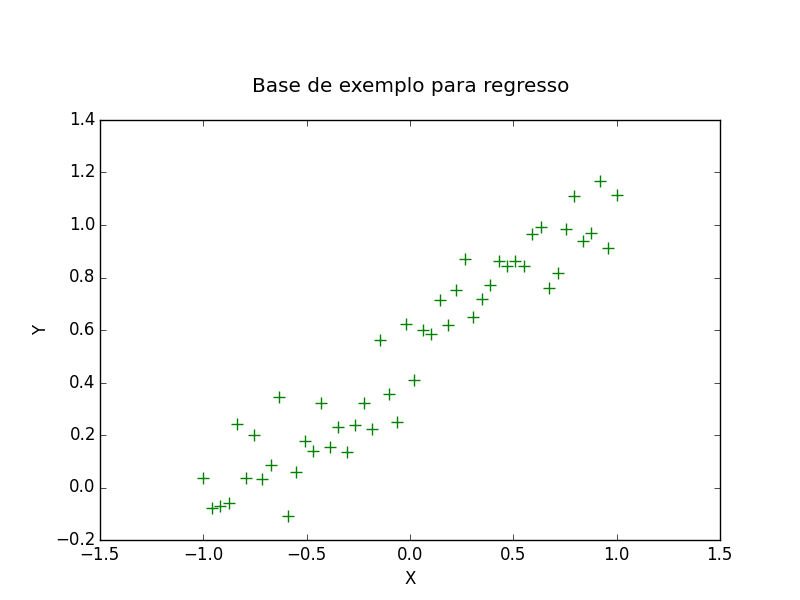
\includegraphics[width=0.40\textwidth]{regression_data_example}
\end{figure}

Para implementar uma solução é, normalmente, necessário assumir alguma função 
com parâmetros desconhecidos $a_{i}$. Os valores desses parâmetros são então 
calibrados para melhor ajuste da função aos dados observados. No caso da 
regressão linear, por exemplo, a saída é assumida como uma função linear da 
entrada, e assim, os parâmetros desconhecidos, $a_{i}$ seriam os coeficientes 
lineares da função.

Ou seja, o problema de regressão pode ser resumido em encontrar um modelo capaz 
de prever corretamente (ou com menor erro possível) o valor da saída do sistema
através do ajuste de parâmetros internos do modelo. A entrada para esse ajuste é 
um conjunto $\{x_{i}, \hat{y}_{i}\}_{i=1}^{p}$. Onde $x_{i}$ é o valor da 
$i$-ésima observação da variável independente $X$ e $\hat{y}_{i}$ é o valor da 
variável dependente $Y$, dado o valor de $X$.

No decorrer deste trabalho, esse problema será tratado utilizando redes neurais 
\acp*{rbf} para relacionar a entrada, $X$ e a saída, $Y$.

\section{Redes RBF}
\label{rbf}


\section{Regressão com redes RBF}
\label{resultados}

\section{Conclusão}
\label{conclusao}

The conclusion goes here.

\section*{Agradecimentos}
We acknowledge the acknowledged acknowledgees.


\bibliography{artigo}
\bibliographystyle{IEEEtran}

\end{document}